\subsection{实验设计}
本实验一共考虑并设计了10个版本的矩阵乘法代码,每个版本都在不同矩阵大小规模和线程数的条件下运行并测量结果,其中实验设计如下:
\begin{table}[h]
\centering
\caption{矩阵乘法优化版本迭代说明}
\begin{tabular}{lll}
\toprule
版本分类          & 核心技术                & 优化逻辑说明 \\
\midrule
基础版[版本0]     & Naive                   & 最原始的$i$-$j$-$k$嵌套,访存步长较大,Cache Miss极高 \\
访存优化[版本1]    & IKJ重排                 & 改变循环顺序,使内层循环对$B$和$C$均为连续内存访问 \\
访存优化[版本2]    & 矩阵转置                & 预先转置矩阵$B$,将纵向访问变为横向连续访问 \\
访存优化[版本3]    & 分块(Blocking)          & 利用分块技术强行提高时间局部性,适配Cache容量 \\
并行优化[版本4]    & 多线程+IKJ              & 将矩阵行拆分给多个线程,并行执行最高效的重排算法 \\
并行优化[版本5]    & 多线程+分块             & 结合线程并行与Cache优化,处理超大规模矩阵 \\
并行优化[版本8]    & 全优化(并行+转置)       & 融合转置带来的访存优势与多线程的计算优势 \\
指令优化[版本6/9]  & 循环展开/向量化         & 减少循环跳转开销,利用编译器自动向量化压榨流水线 \\
指令优化[版本10]  & 手动AVX2(仅WSL)         & 手动调用Intel指令集,单指令多数据并行处理 \\
\bottomrule
\end{tabular}
\end{table}

\subsection{实验过程}
编写对应各个版本矩阵乘代码,考虑到模拟环境性能较差,运行速度较慢,所以首先在宿主机WSL2(Arch Linux)上运行测试(考虑到不同版本的代码在不同平台测试结果相差较大,但在仙女沟通平台应呈现出一致的趋势).
实验过程截图如图:
\begin{table}[H]
    \centering
    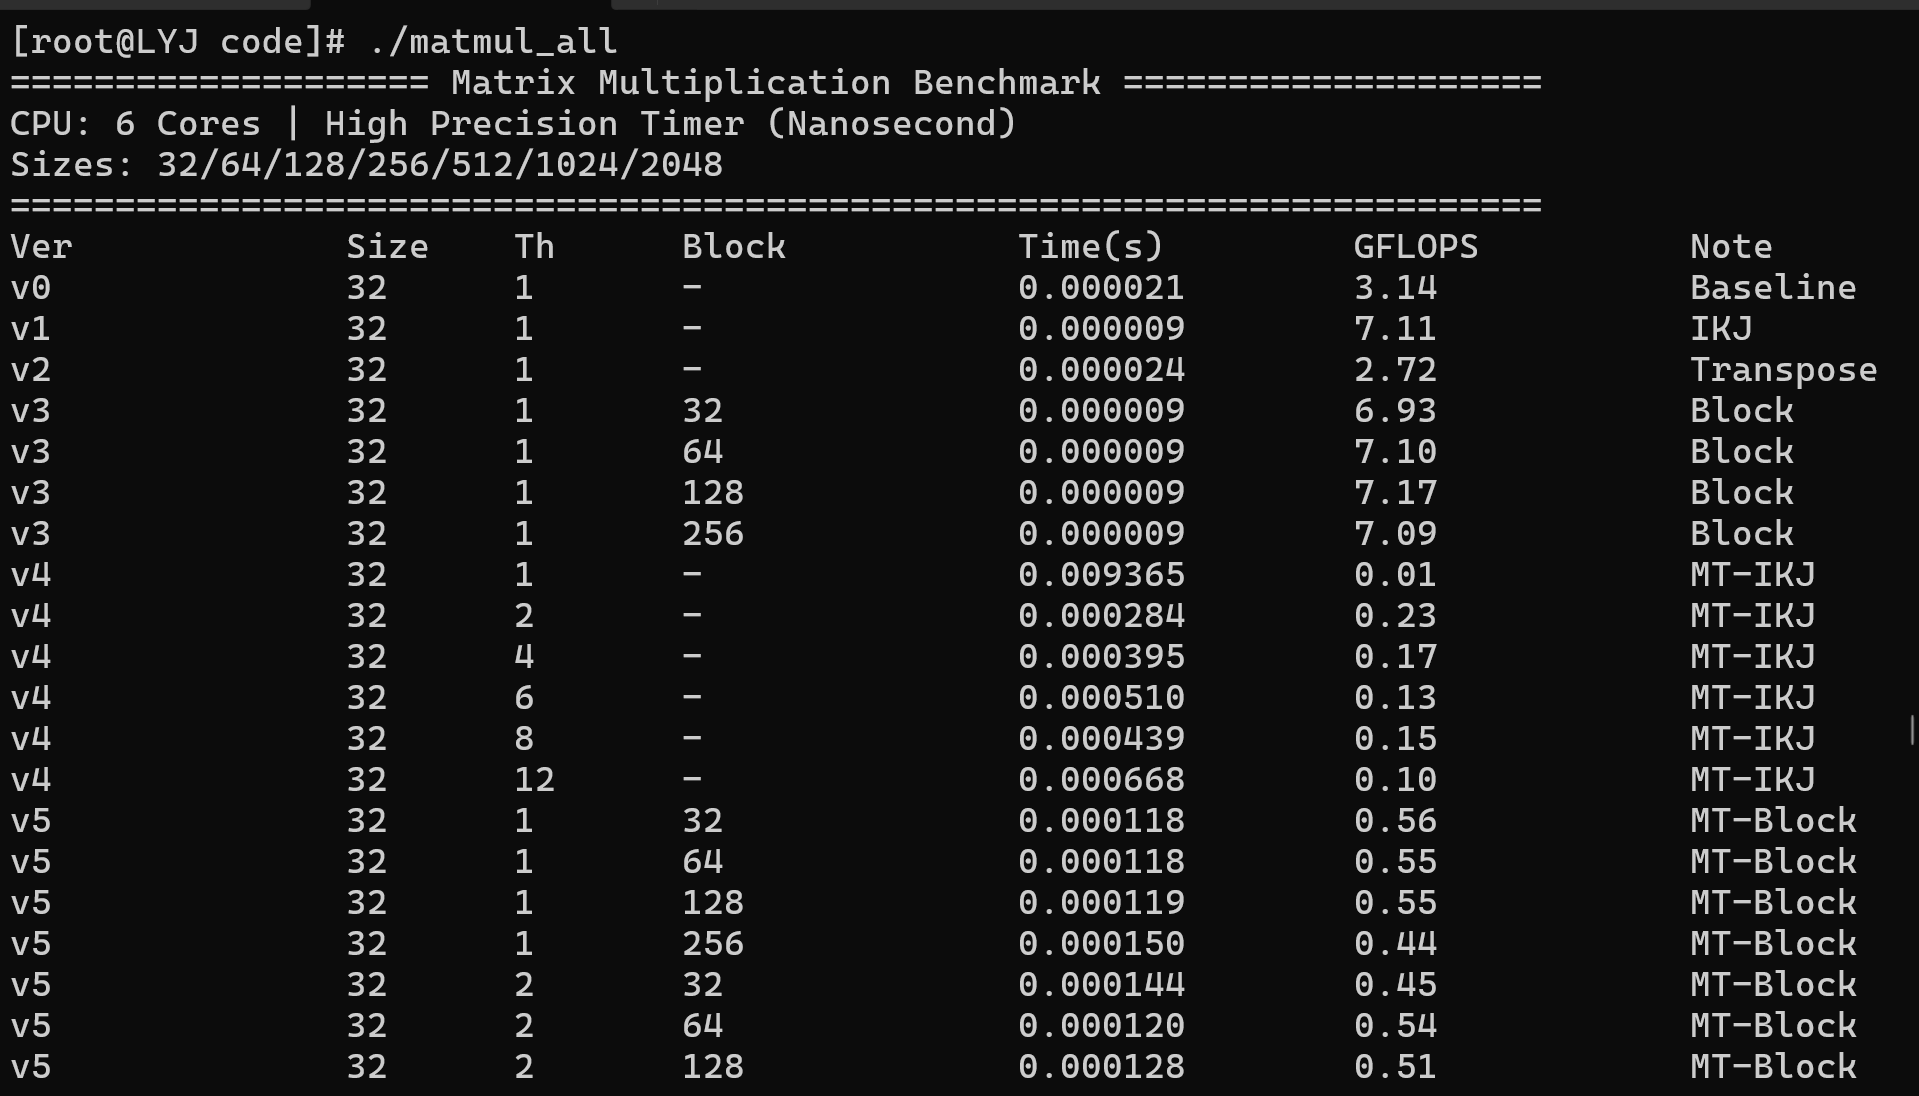
\includegraphics[width = 1\textwidth]{figure/task1_wsl.png}
    \caption{实验一运行过程截图(宿主机)}
\end{table}

实验代码在宿主机上成功运行得到准确数据后,迁移至VMware的ubuntu虚拟机上,在QEMU环境上测试运行。由于软件模拟导致性能远小于在宿主机上运行,因此适当减小了
实验数据,并删去了X86特有的AVX2指令集,实验过程截图如图:
\begin{table}[H]
    \centering
    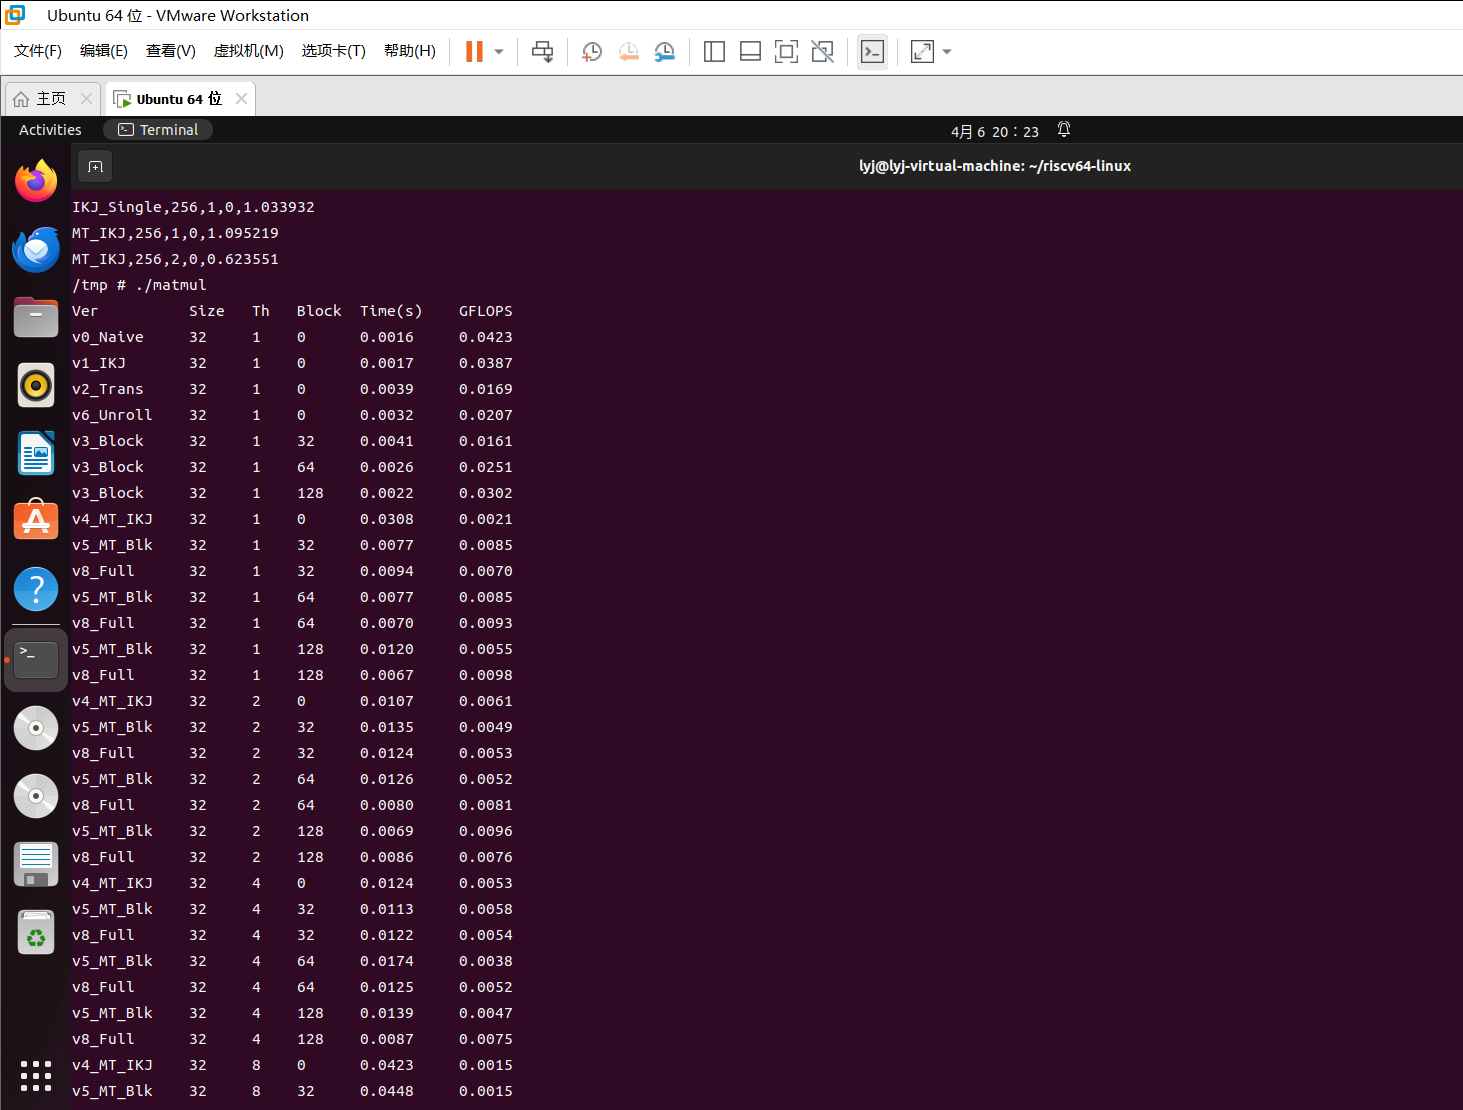
\includegraphics[width = 1\textwidth]{figure/task1_vmware.png}
    \caption{实验一运行过程截图(VMware)}
\end{table}



\subsection{实验结果}
不同优化版本的矩阵乘法代码在各种测试条件下(输入规模大小、并行线程数、分块大小)在WSL2(Arch Linux)上运行结果绘制成折线图如图:
\begin{figure}[H]
    \centering
    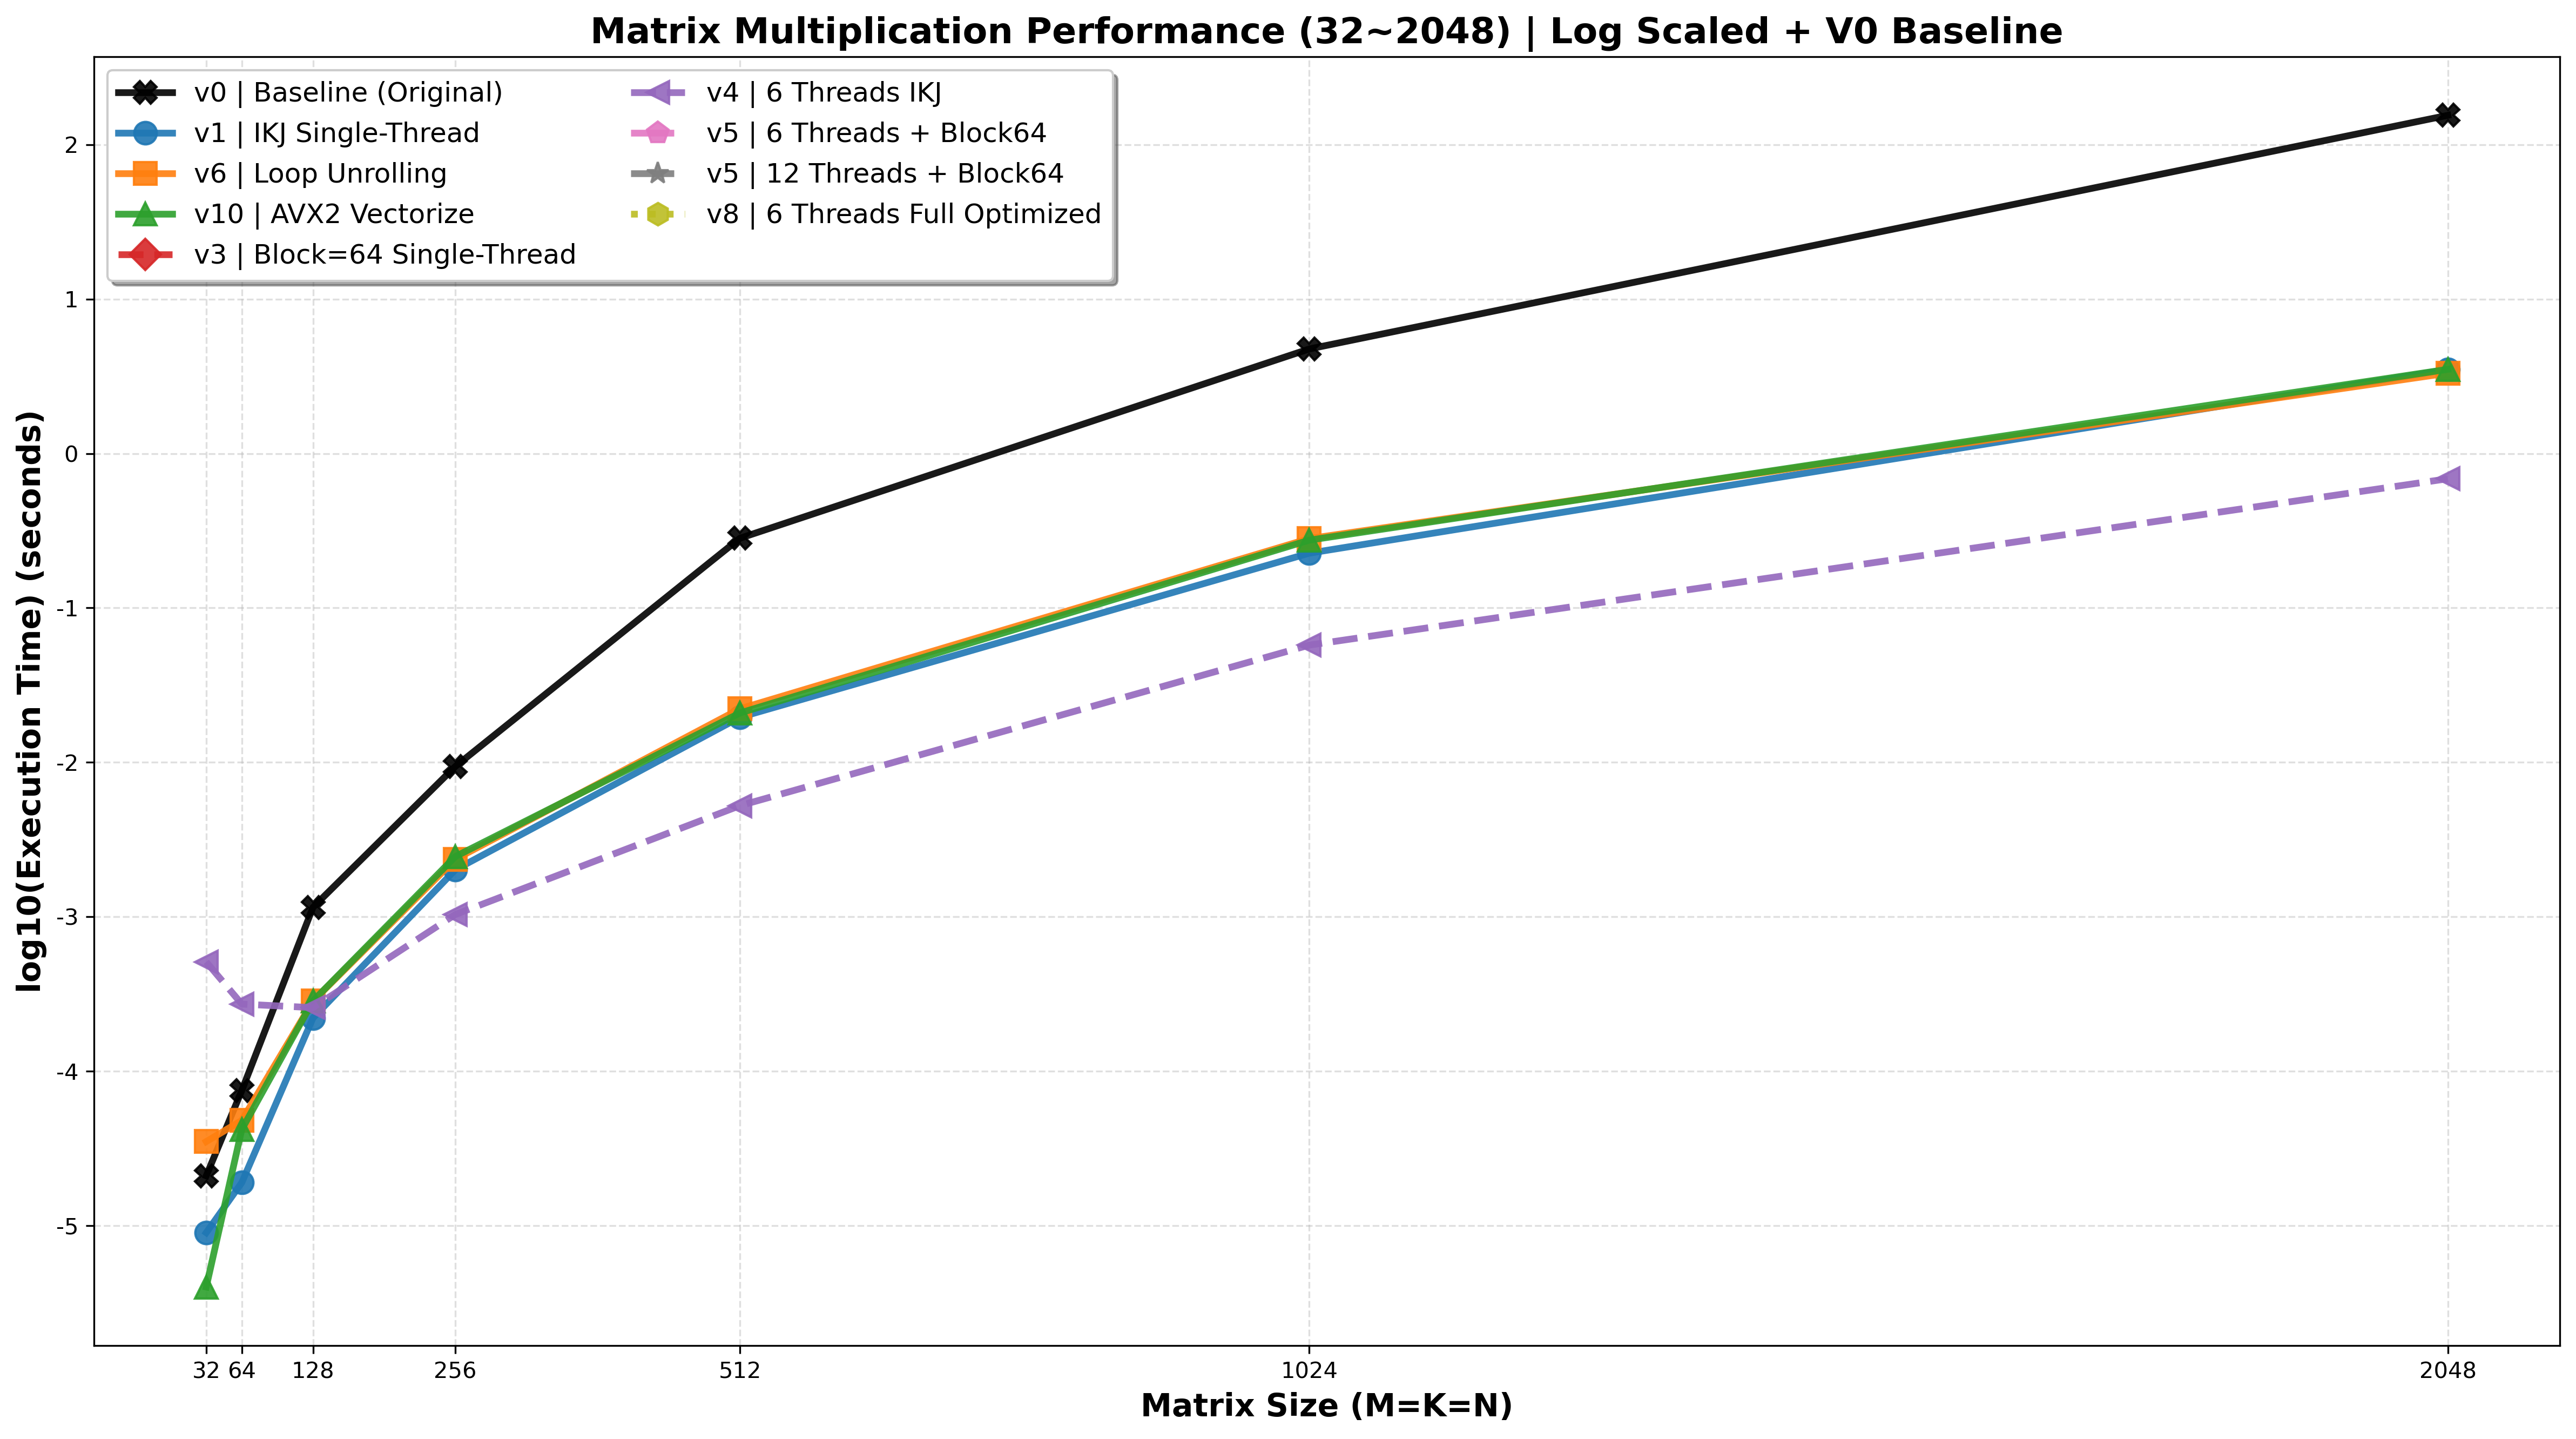
\includegraphics[width = 1\textwidth]{figure/matrix_performance_with_v0_log.png}
    \caption{实验一运行结果折线图(宿主机)}
\end{figure}
其中纵坐标为对应运行时间取对数。
相应的修改代码在QEMU模拟环境上运行结果绘制成折线图如图:
\begin{figure}[H]
    \centering
    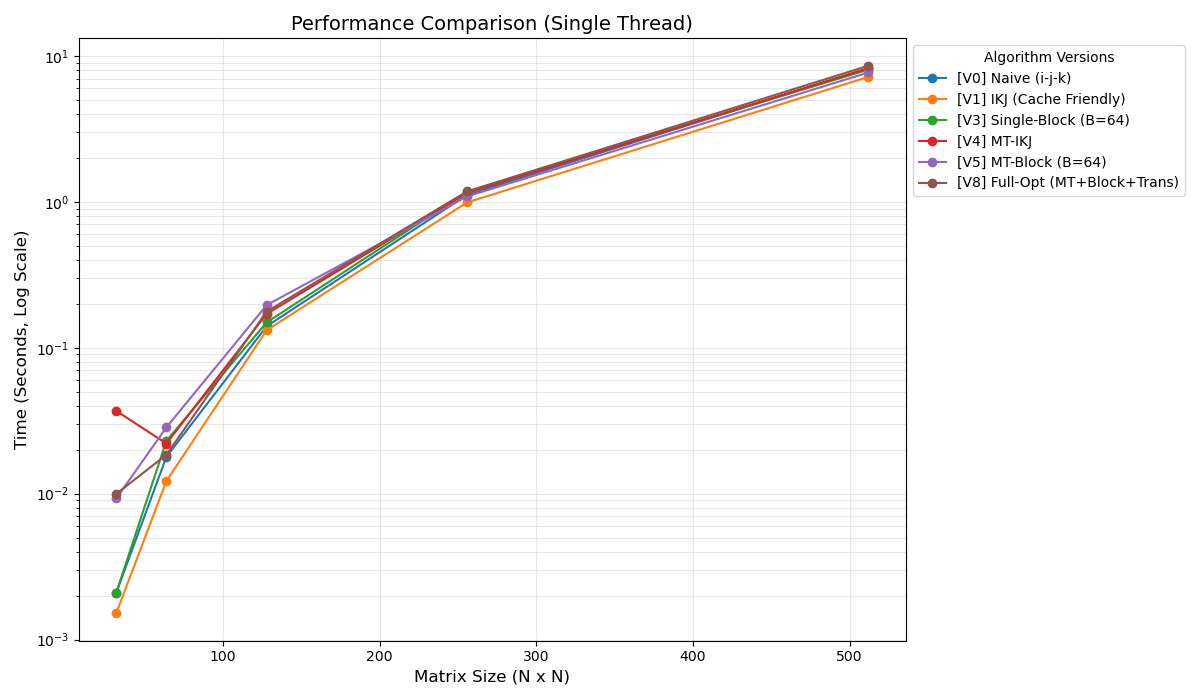
\includegraphics[width = 1\textwidth]{figure/single_thread_comparison.png}
    \caption{实验一运行结果折线图(VMware)}
\end{figure}
\begin{figure}[H]
    \centering
    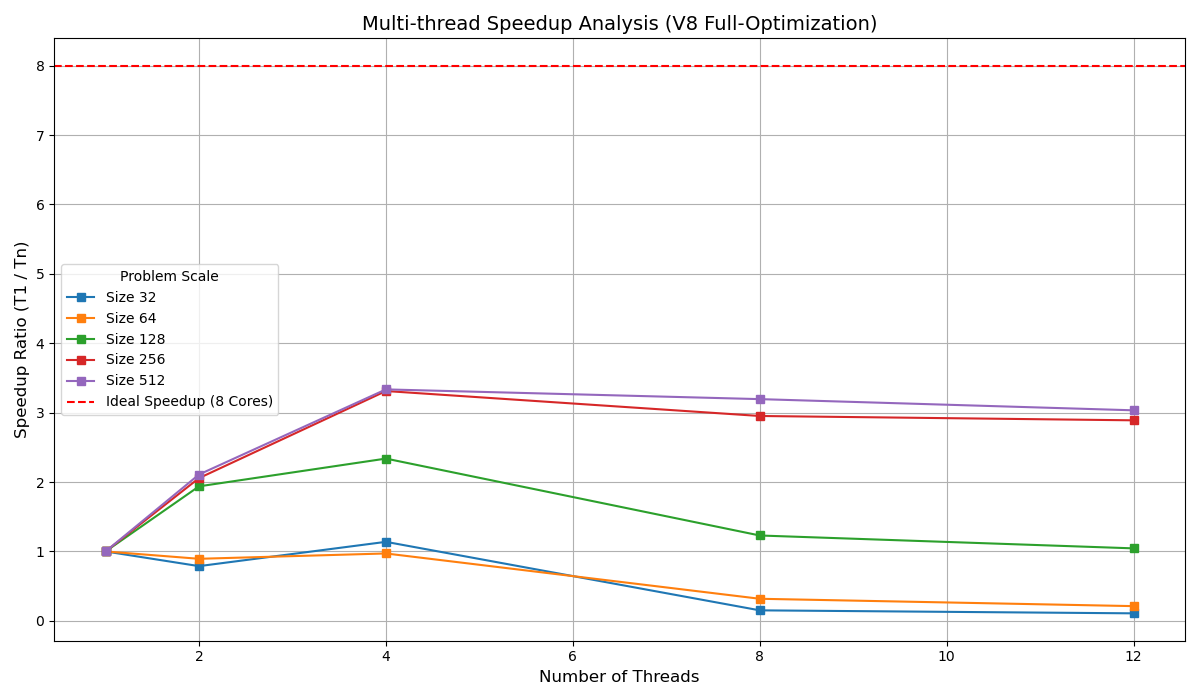
\includegraphics[width = 1\textwidth]{figure/speedup_analysis_v8.png}
    \caption{实验一加速比}
\end{figure}

从两种环境下的运行结果图片可以看出,各优化版本的性能较原始版本相比都有了很大的提升

